\documentclass[a4paper,12pt]{article} 
\usepackage[T2A]{fontenc}			
\usepackage[utf8]{inputenc}			
\usepackage[english,russian]{babel}	
\usepackage{amsmath,amsfonts,amssymb,amsthm,mathrsfs,mathtools} 
\usepackage{cancel}
\usepackage{multirow}
\usepackage[colorlinks, linkcolor = blue]{hyperref}
\usepackage{upgreek}\usepackage[left=2cm,right=2cm,top=2cm,bottom=3cm,bindingoffset=0cm]{geometry}
\usepackage{tikz}
\usepackage{graphicx}
\usepackage{subfig}
\usepackage{titletoc}
\usepackage{pgfplots}
\usepackage{xcolor}
\usepackage{wrapfig}
\author{Дорогинин Д.В.\\
Группа Б02-825}
\title{Д4.2 Изучение поглощения света в жидкости.}
\date{}

%\begin{wrapfigure}{r}{0.5\textwidth}
%\begin{center}
%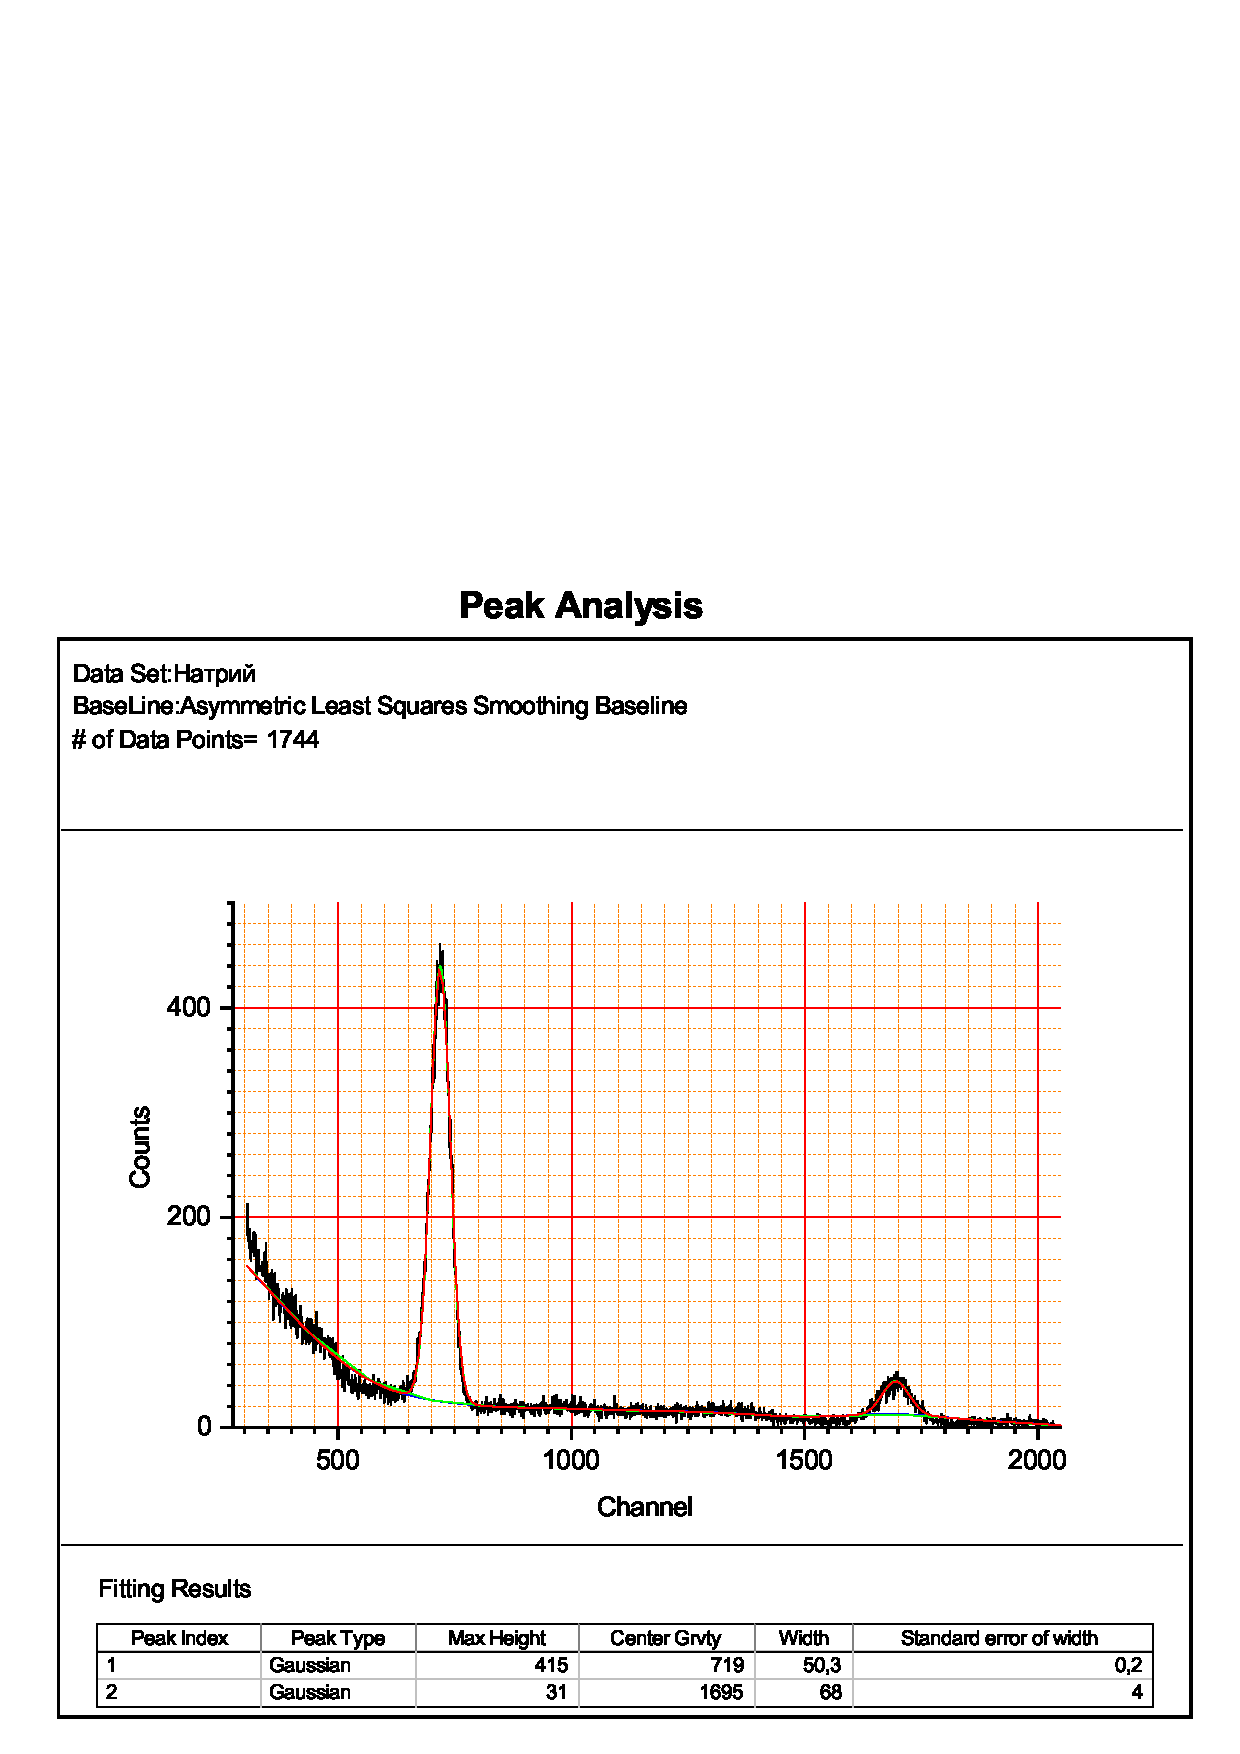
\includegraphics[width = 0.4\textwidth]{1.png}
%\end{center}
%\caption{}
%\end{wrapfigure}

%\begin{wrapfigure}{r}{0.5\textwidth}
%\begin{center}
%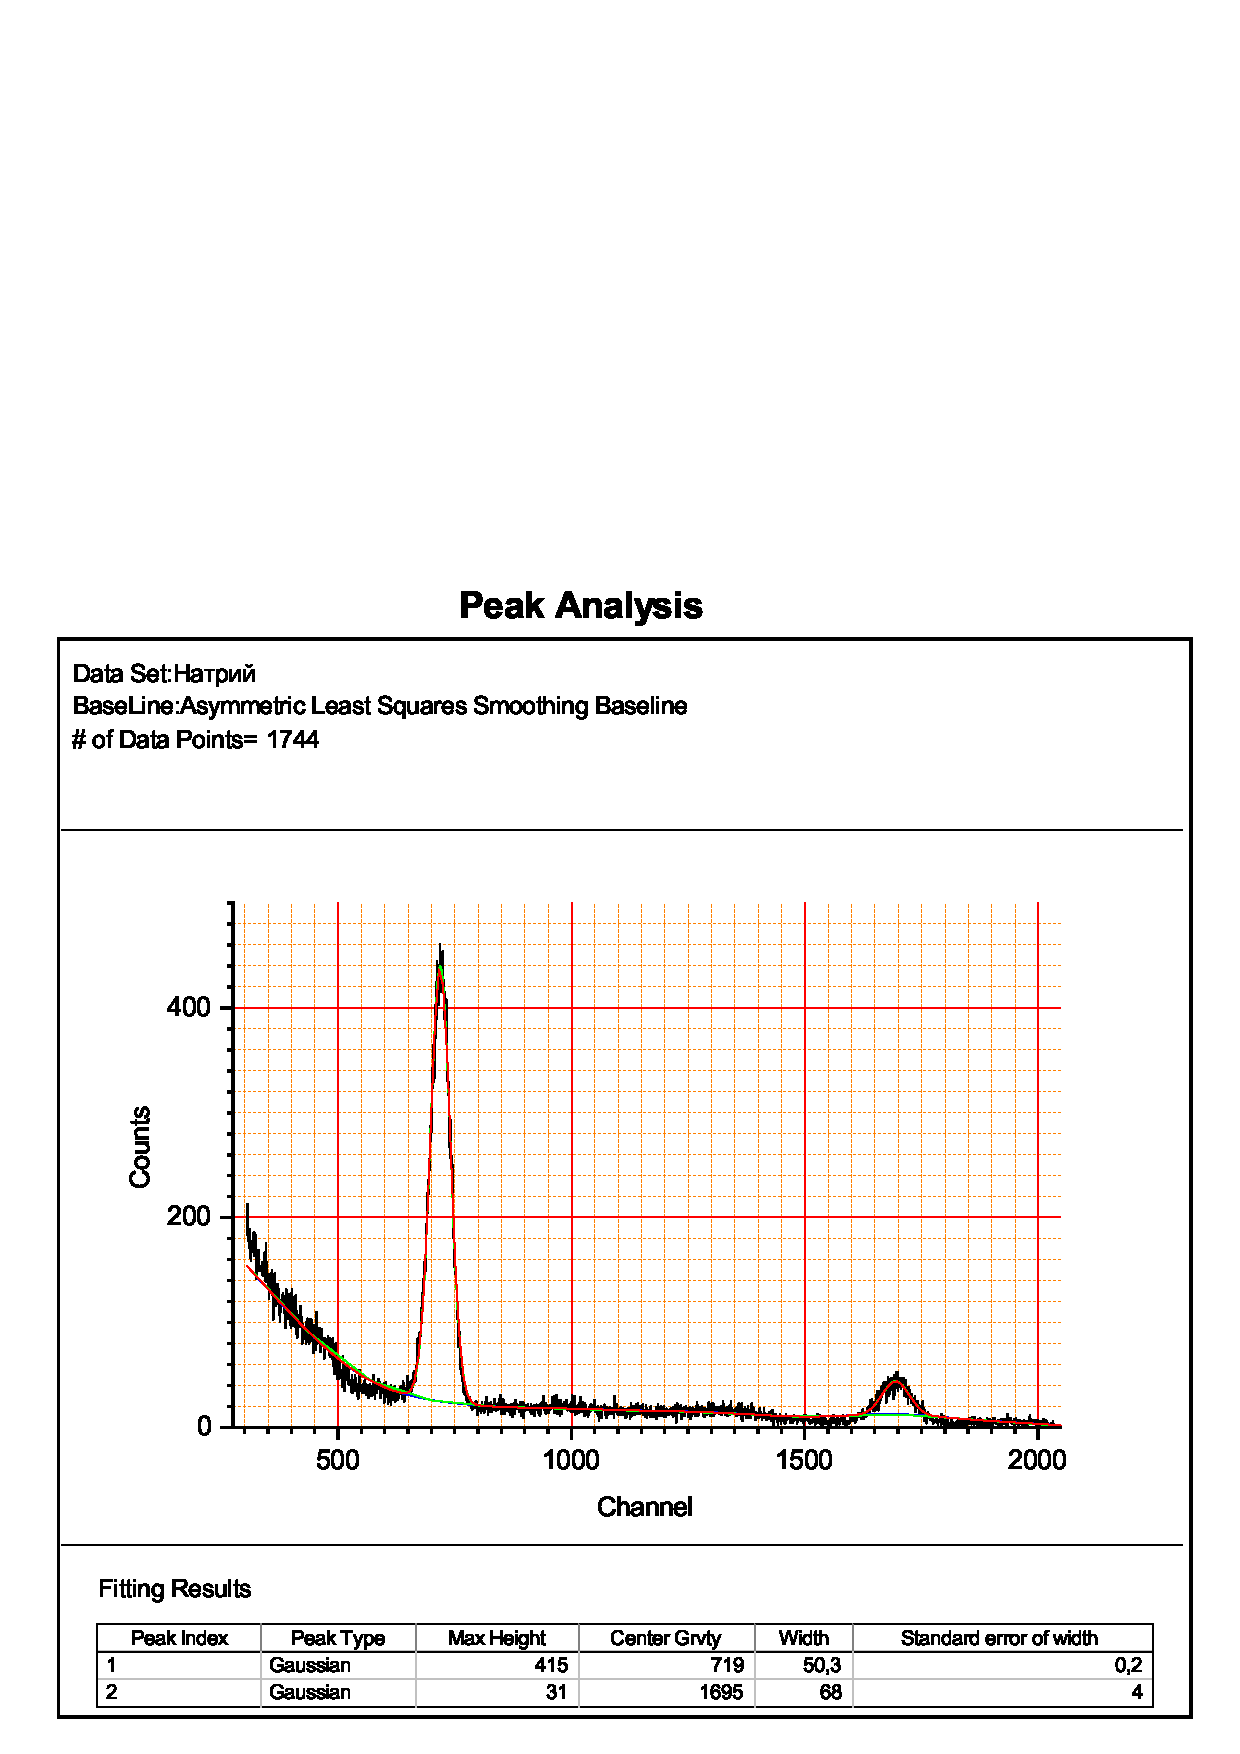
\includegraphics[width = 0.4\textwidth]{1.png}
%\end{center}
%\caption{}
%\end{wrapfigure}

\begin{document}
\maketitle
\textbf{Цель работы}: экспериментнально проверить закон Ламберта-Бугера-Бера и измерить коэффициент поглощения крепкого чайного настоя.


\textbf{В работе используются}: лазерная указка, ваза, линейка, настой чайных листьев, камера, графический редактор Krita.
\section*{Теория}
Пусть свет проходит через вещество, взаимодействуя с $N$ молекулами, имеющими шанс $p$ захватить. Тогда изменение числа фотонов
$$
dN_{\text{ф}} = -pN_{\text{ф}} dN.
$$
Для изменения интенсивности этого потока, в предположении $I = \beta N_{\text{ф}}$ ($\beta$ -- коэффициент пропорциональности), подающего на плоский слой толщиной $dx$ и площадью $S$, справедливо 
$$
dI = \dfrac{pnS}{\beta} I dx = -\alpha I dx,
$$
где $n$ -- концентрация молекул. Коэффициент $\alpha$ -- \textit{коэффициент поглощения}. Интегрируя это выражения получим \textit{закон Ламберта-Бугера-Бера}:
\begin{equation}
I = I_0 e^{-\alpha x}
\end{equation} 
\begin{figure}[h]
\begin{minipage}[h]{0.6\linewidth}
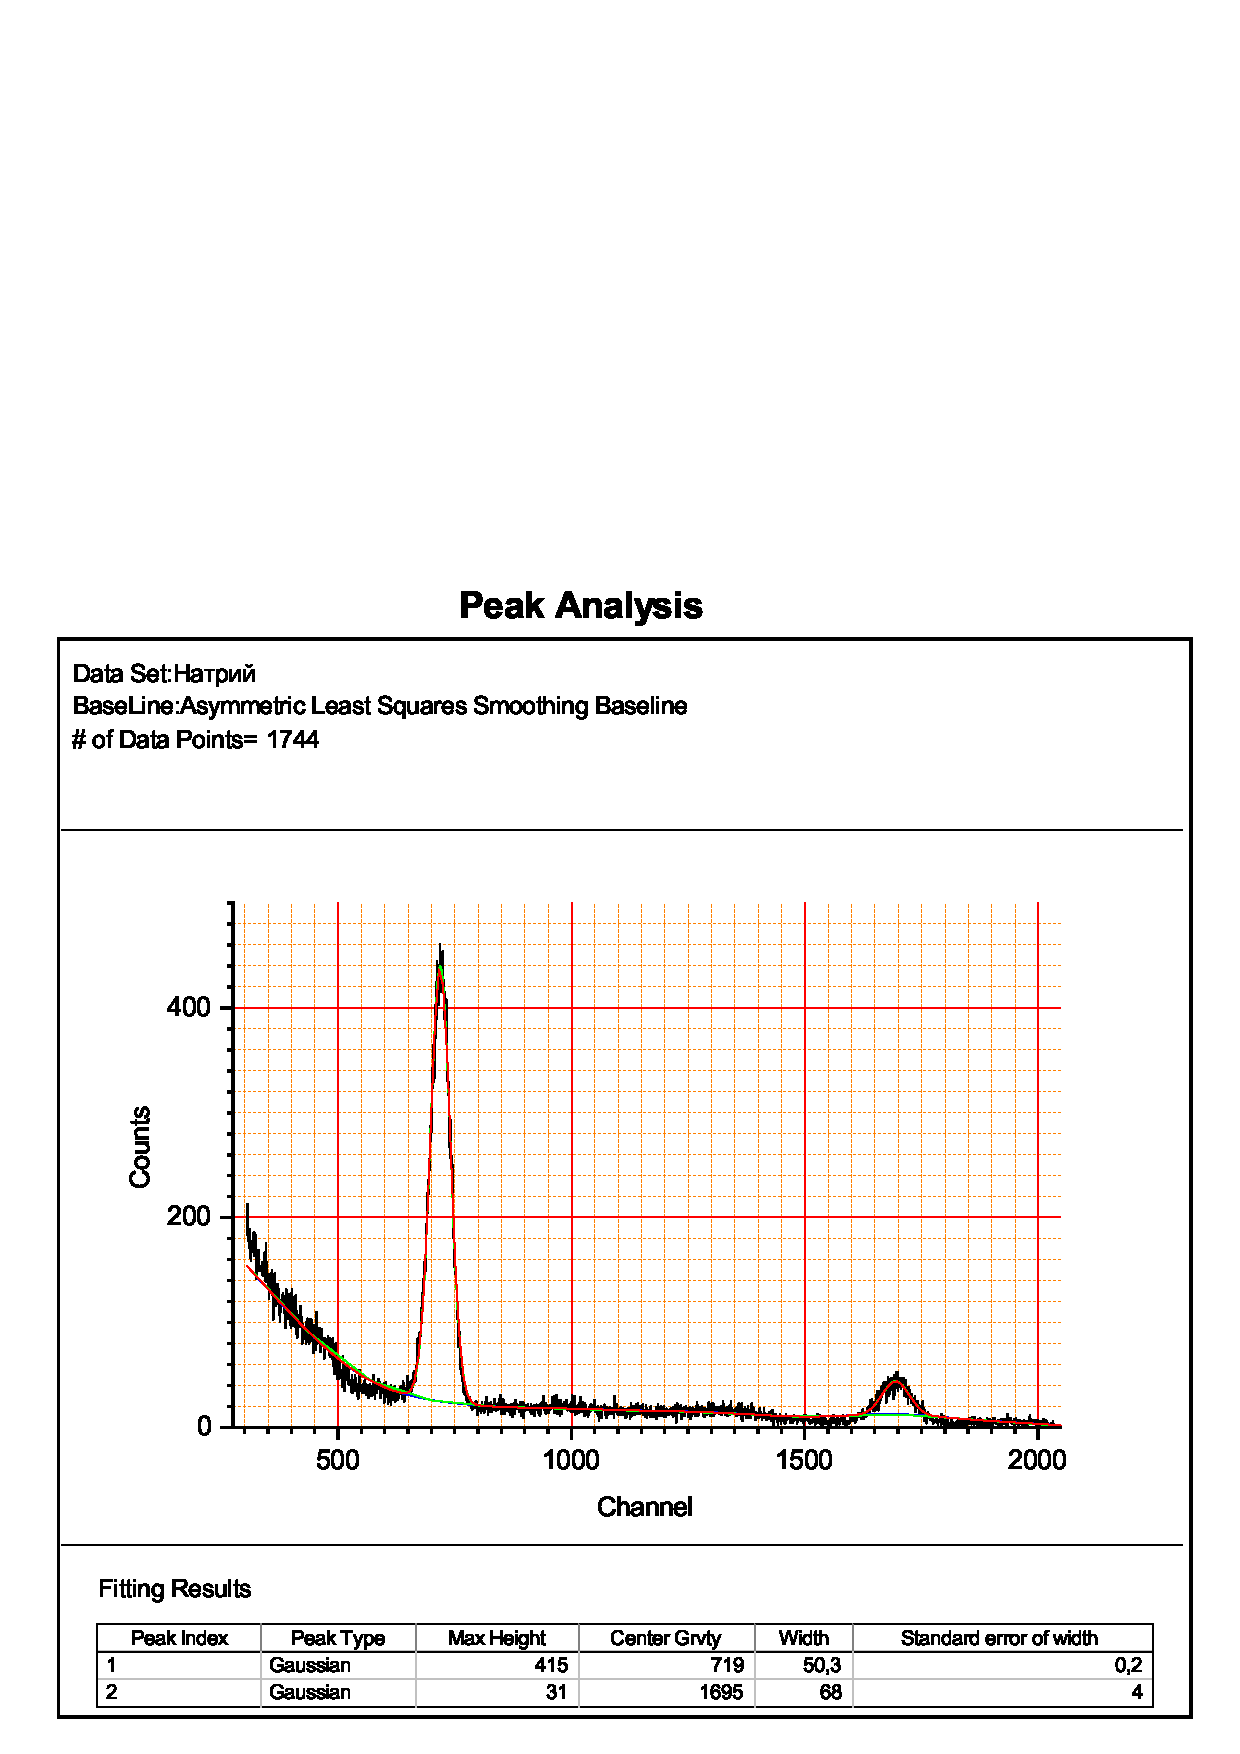
\includegraphics[scale=0.6]{1.png}
\centering
\end{minipage}
\hfill
\begin{minipage}[h]{0.4\linewidth}
\includegraphics[scale=0.09]{4.png}
\end{minipage}
\caption{Схема установки и пример изображения.}
\end{figure}

На Рис. 1 представлена схема установки. Ваза заполняется исследуемой жидкостью до высоты $h$ и помещается в тёмное место. Сверху ваза освещается лазером Л. Делается снимок полученного на дне станака пятна камерой Ф, который далее анализируется в редакторе фотографий: на изображении пятна находится пиксель с интенсивностью света, близкой к максимальной в пятне, и его интенсивность $i$ фиксируется. Здесь за интенсивность пикселя принимаем величину
$$
i = \dfrac{i_R + i_G + i_B}{3},
$$
где $i_R$, $i_G$ и $i_B$ -- интенсивности света базовых цветов пикселя. Эта интенсивность пропорциональна исследуемой $i \propto I$. Так как свет проходит через чайный настой дважды, то
$$
I \propto e^{-2\alpha h}.
$$
Для исследования зависимости концентрации чайного настоя $n = n(t)$ от времени заваривания использовался одинаковый объём воды одинаковой температуры и одинаковое количество чайных листьев для каждого заваривания.
\section*{Ход работы}
Собираем установку, измерения для разных температур и высот представлены в Таблице 1. 
\begin{table}[h]
\begin{tabular}{|c|c|c|c|c|c|c|c|}
\hline
$t$, мин              & 5               & $t$, мин & 10  & $t$, мин     & 15     & $t$, мин & 20  \\ \hline \hline
$h$, см               & $i$             & $h$, см  & $i$ & $h$, см      & $i$    & $h$, см  & $i$ \\ \hline
2.0                   & 255             & 3.0      & 247 & 5.0          & 247    & 4.0      & 246 \\ \hline
18.0                  & 230             & 6.0      & 246 & 8.0          & 244    & 8.0      & 241 \\ \hline
20.0                  & 212             & 9.5      & 243 & 11.0         & 157    & 10.5     & 243 \\ \hline
22.5                  & 188             & 14.0     & 242 & 15.0         & 153    & 12.5     & 138 \\ \hline 
\multicolumn{2}{|c|}{\multirow{4}{*}{}} & 16.5     & 222 & 17.5         & 97     & 15.0     & 132 \\ \cline{3-8} 
\multicolumn{2}{|c|}{}                  & 18.5     & 198 & 20.5         & 48     & 18.5     & 77  \\ \cline{3-8} 
\multicolumn{2}{|c|}{}                  & 20.5     & 163 & 22.0         & 43     & 20.5     & 87  \\ \cline{3-8} 
\multicolumn{2}{|c|}{}                  & 22.0     & 121 & \multicolumn{2}{c|}{} & 22.0     & 38  \\ \hline
\end{tabular}
\centering
\caption{Результаты изменения.}
\end{table}\\
Результаты представим на графике (Рис. 2) в осях $\left(\ln\left( \dfrac{i}{i_0} \right), 2h\right)$, где $i_0$ -- яркость при минимальной высоте настоя. На графиках точки начинаются с момента, когда яркость пятна начинает меняться.
\newpage
\begin{figure}
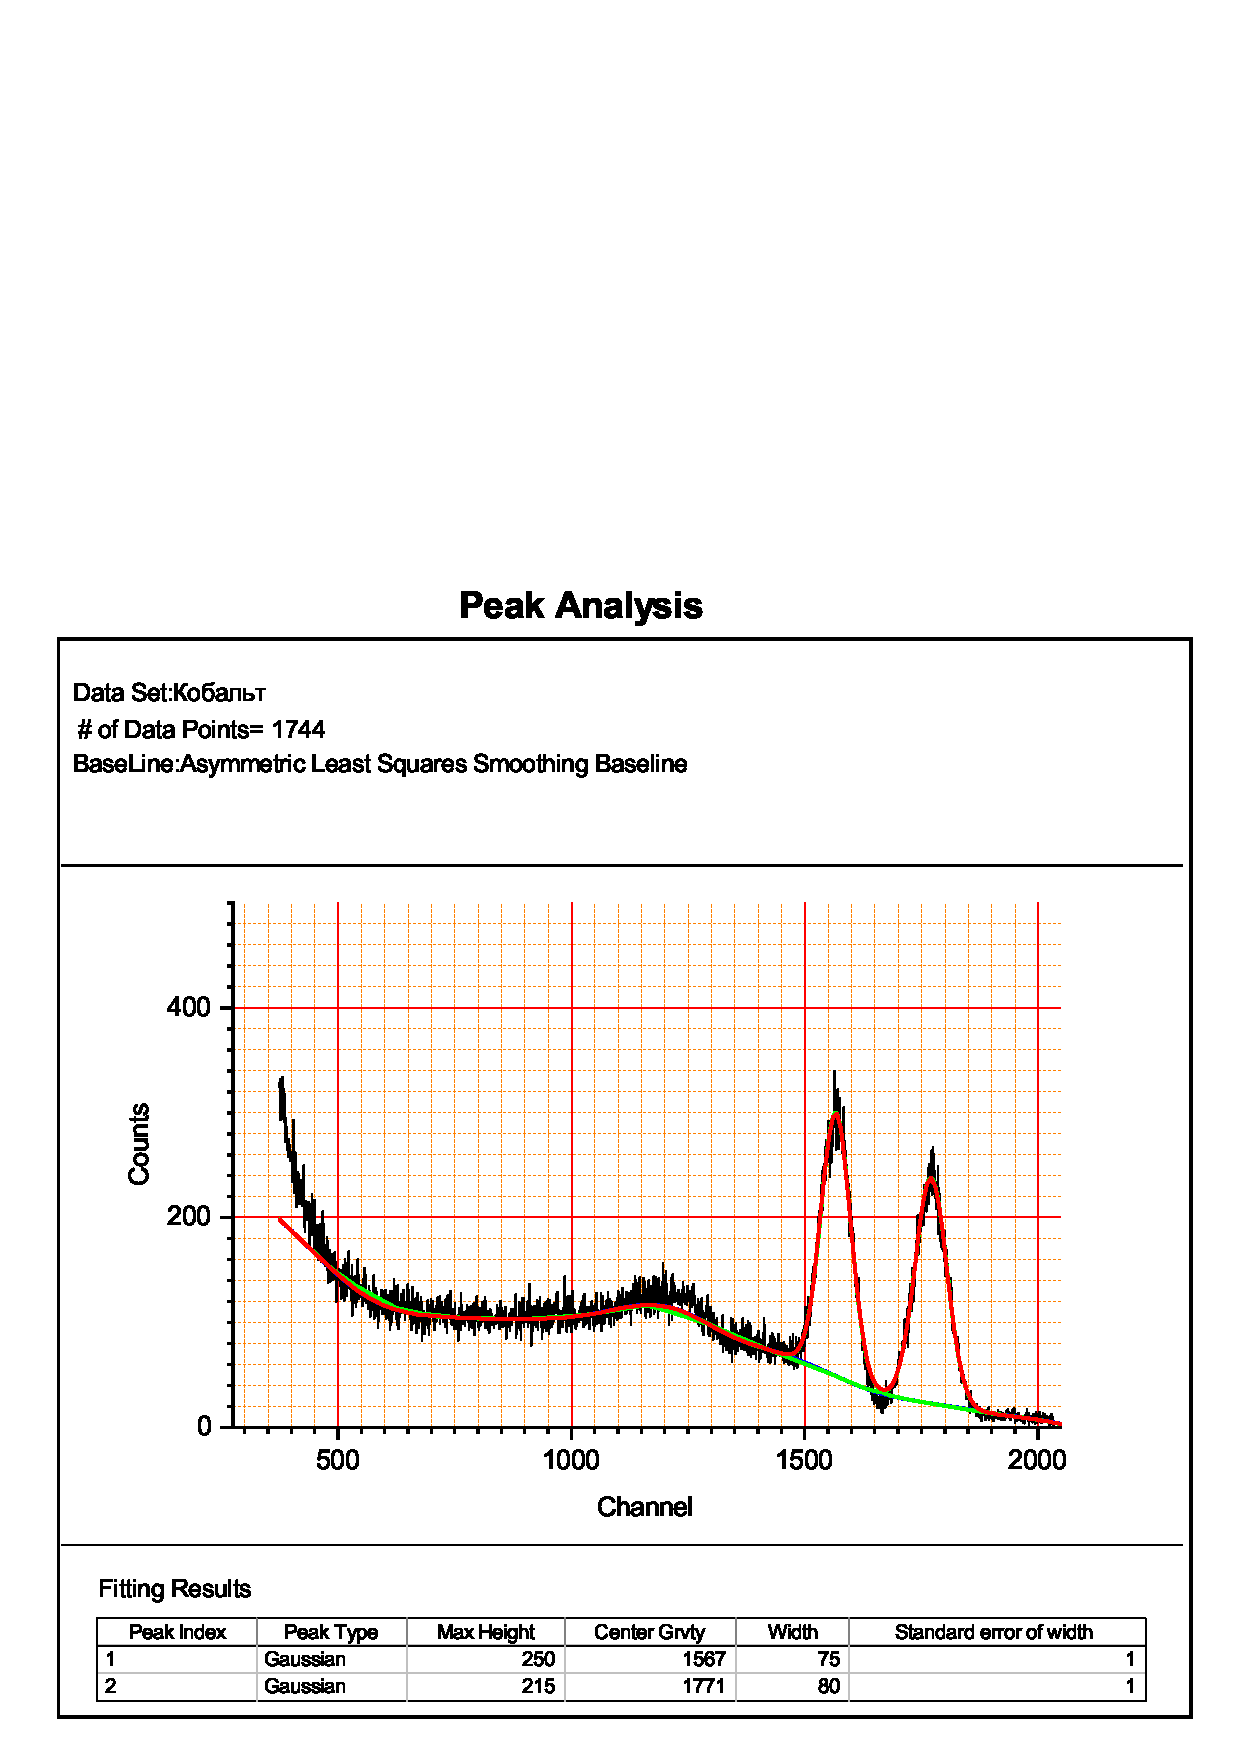
\includegraphics[scale=0.4]{2.png}
\centering
\caption{Зависимости $\ln\left( \dfrac{i}{i_0} \right) = \left(\ln\left( \dfrac{i}{i_0} \right)\right) [2h]$ для $t = 5,~10,~15,~20 \text{ мин}$.}
\end{figure}
Результаты измерений для $\alpha$ представлены в Таблице 2. Таким образом, закон Ламберта-Бугера-Бера выполняется. Представим зависимость $\alpha = \alpha(t)$ на графике (Рис. 2). Из графика можно предположить, что зависимость имеет вид $\alpha \propto 1 - e^{-Ct}$, а так как $\alpha \propto n$, тот же закон будет выполняться и для концентрации. Высокая погрешность измерений и их малое количество не позволяют проверить зависимость точнее.
\begin{figure}[h]
\begin{minipage}[h]{0.4\linewidth}
\begin{tabular}{|c|c|c|}
\hline
$t$, мин & $\alpha$, $\text{с}^{-1}$ & $\sigma_\alpha$, $\text{с}^{-1}$ \\ \hline
5   & 0.023    & 0.010           \\ \hline
10  & 0.045    & 0.011           \\ \hline
15  & 0.062    & 0.009           \\ \hline
20  & 0.064    & 0.012           \\ \hline
\end{tabular}
\centering
\end{minipage}
\hfill
\begin{minipage}[h]{0.7\linewidth}
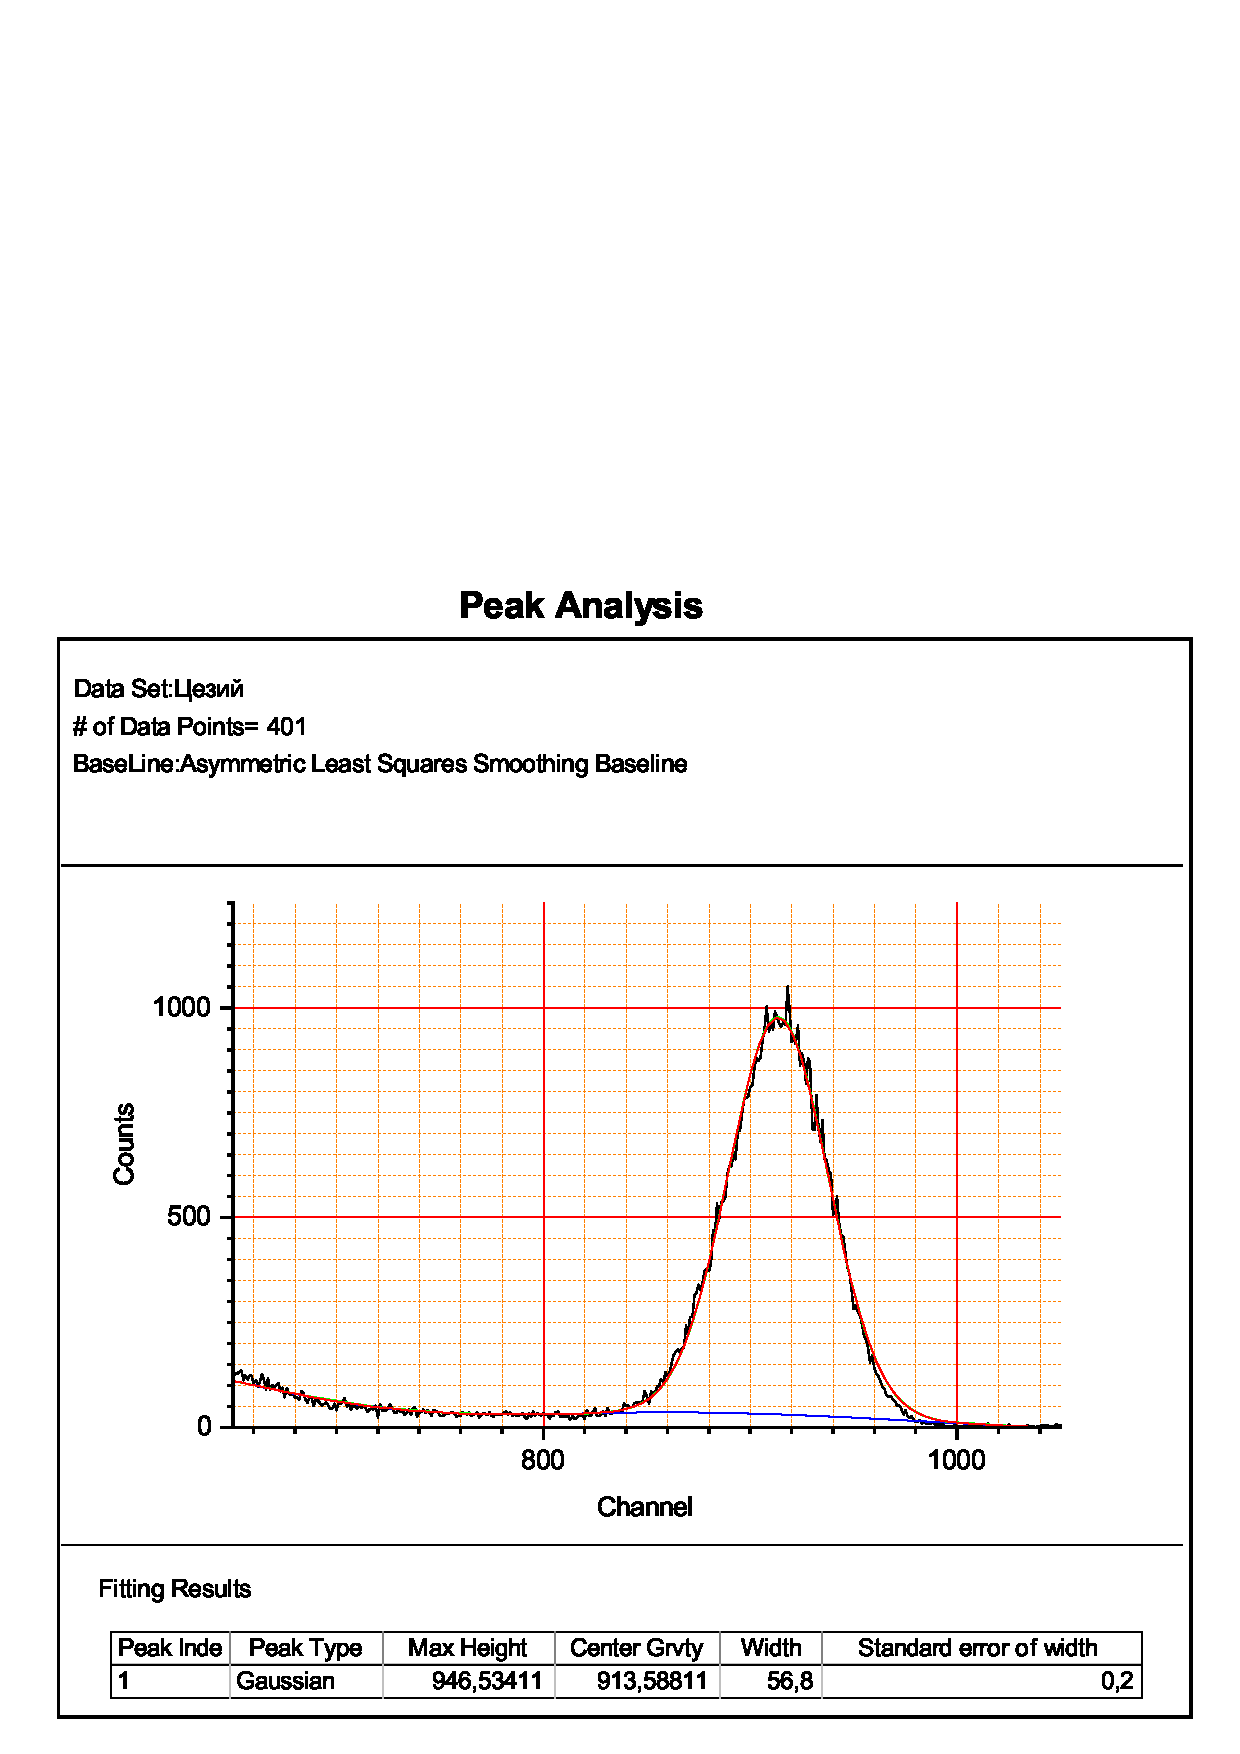
\includegraphics[scale=0.7]{3.png}
\end{minipage}
\caption{Результаты измерений и зависимость $\alpha = \alpha(t)$.}
\vspace{-20pt}
\end{figure}
%
%\begin{table}[h]
%\begin{tabular}{|c|c|c|c|c|}
%\hline
%$t$             & 5      & 10    & 15    & 20    \\ \hline
%$\alpha$        & 0.0225 & 0.045 & 0.062 & 0.064 \\ \hline
%$\sigma_\alpha$ & 0.010  & 0.011 & 0.009 & 0.012 \\ \hline
%\end{tabular}
%\centering
%\caption{Данные для зависимости $\alpha = \alpha(t)$.}
%\end{table}
%\begin{figure}
%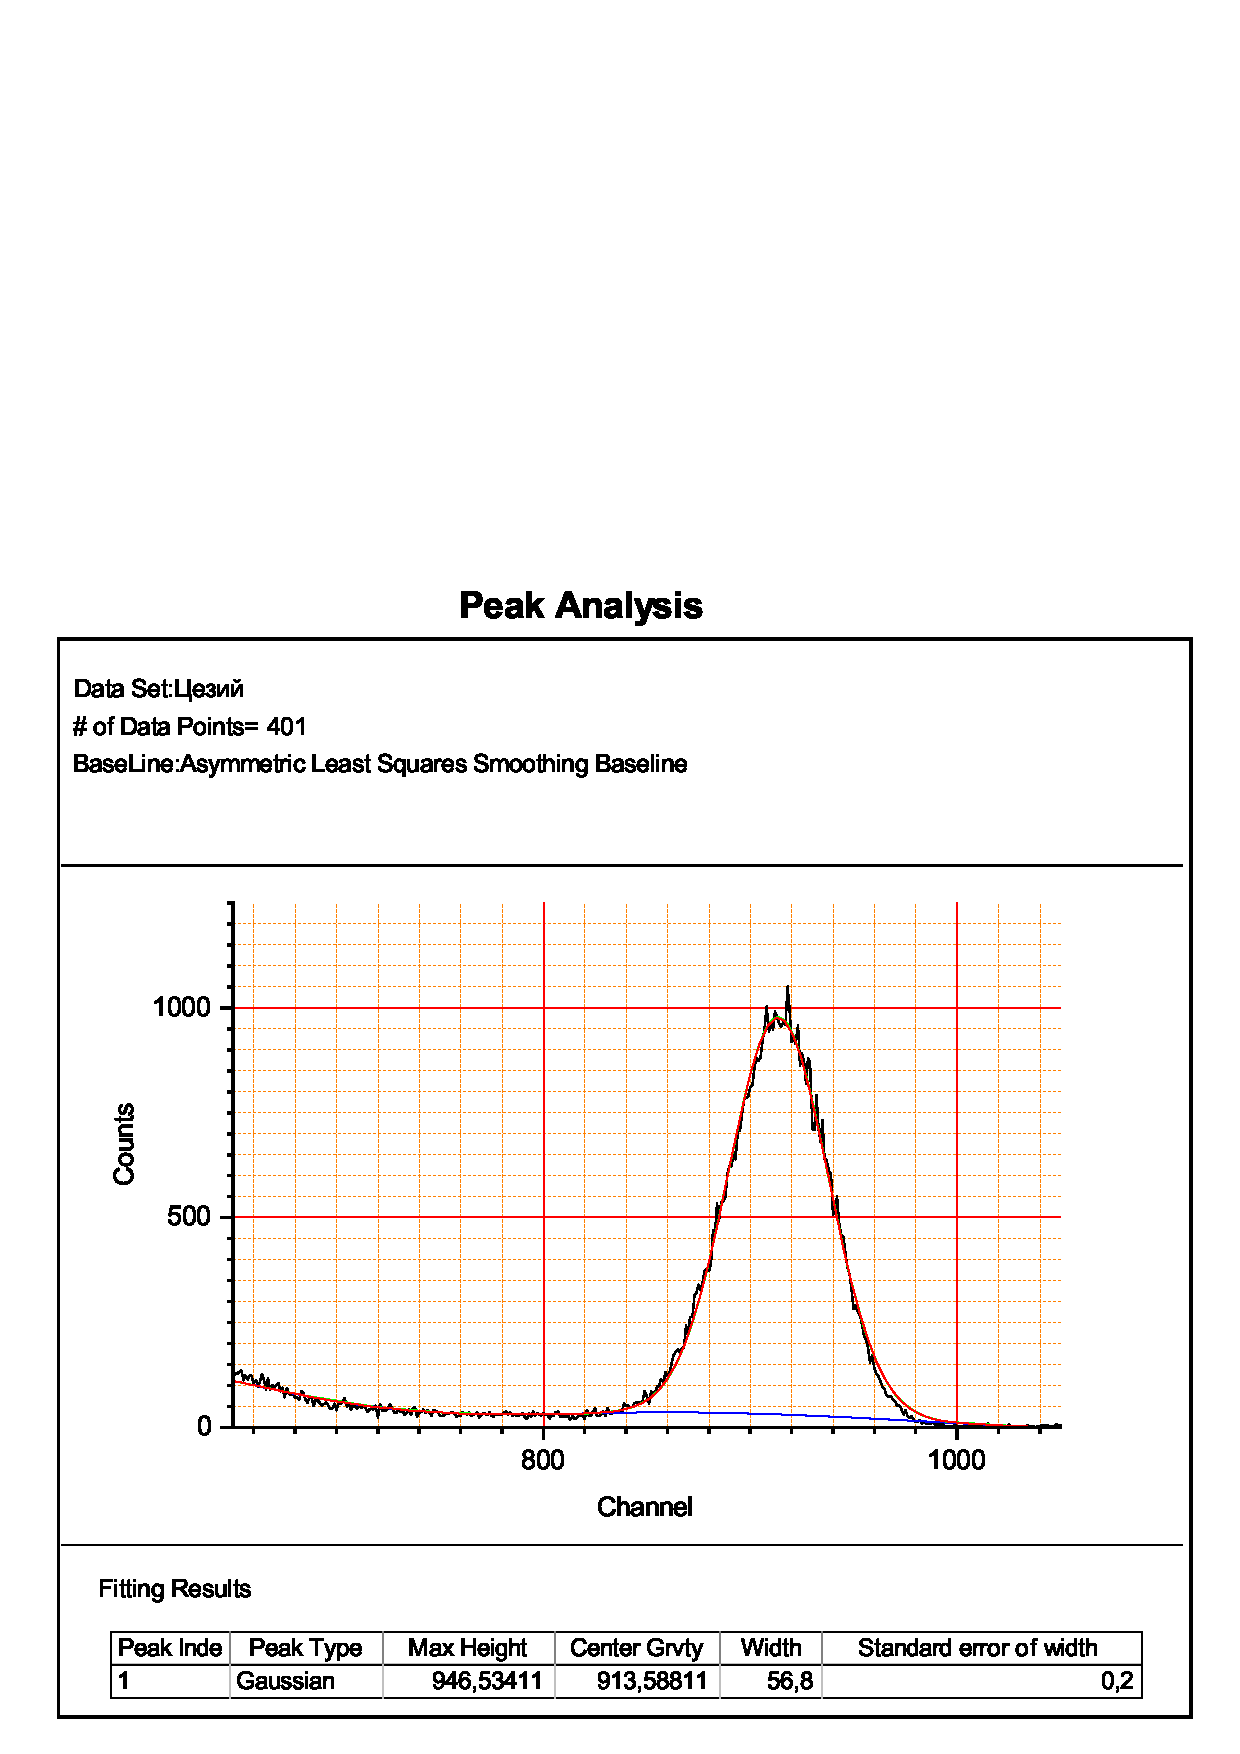
\includegraphics[scale=0.5]{3.png}
%\centering
%\caption{Зависимости $\alpha = \alpha(t)$.}
%\end{figure}
\end{document}